% THIS DOCUMENT IS FOLLOWS THE VOLERE TEMPLATE BY Suzanne Robertson and James Robertson
% ONLY THE SECTION HEADINGS ARE PROVIDED
%
% Initial draft from https://github.com/Dieblich/volere
%
% Risks are removed because they are covered by the Hazard Analysis
\documentclass[12pt]{article}

\usepackage{booktabs}
\usepackage{tabularx}
\usepackage{hyperref}
\usepackage{float}
\usepackage{graphicx}
\usepackage{tikz}
\usepackage{tikz-uml}
\usepackage{tabularray}
\usepackage{xcolor}

\hypersetup{
    bookmarks=true,         % show bookmarks bar?
      colorlinks=true,      % false: boxed links; true: colored links
    linkcolor=red,          % color of internal links (change box color with linkbordercolor)
    citecolor=green,        % color of links to bibliography
    filecolor=magenta,      % color of file links
    urlcolor=cyan           % color of external links
}

% ~~~~~~~ Glossary Content Goes Here ~~~~~~~

\usepackage[nonumberlist, nopostdot, nogroupskip]{glossaries}

% Define custom glossary types 
\newglossary[slg]{SWE}{swd}{swi}{Software Engineering Terms}
\newglossary[dlg]{domain}{dld}{dli}{Domain-Specific Research Terms}
\newglossary[glg]{general}{gld}{gli}{General Terms}

% Make glossaries
\makenoidxglossaries
 
% Software Engineering Related Technical Terms 

\newglossaryentry{api}{
    type=SWE,
    name={API}, 
    description={An interface or set of rules that allow different software systems to communicate with each other.}
}

\newglossaryentry{backend}{
    type=SWE,
    name={Backend}, 
    description={The server-side part of the system responsible for business logic, data processing, storage and retrieval.}
}

\newglossaryentry{frontend}{
    type=SWE,
    name={Frontend}, 
    description={The part of the system that the user interacts with (e.g. the website interface)}
}

\newglossaryentry{nlp}{
    type=SWE,
    name={Natural Language Processing (NLP)},
    description={A field of artificial intelligence that enables machine interpretation of human language.}
}

\newglossaryentry{database-schema}{
    type=SWE,
    name={Database Schema},
    description={The structure of a database, including tables, fields, and relationships}
}

\newglossaryentry{data-pipeline}{
    type=SWE,
    name={Data Pipeline},
    description={A sequence of data processing steps that transform raw inputs into usable outputs}
}

\newglossaryentry{metadata}{
    type=SWE,
    name={Metadata},
    description={Descriptive information about a dataset, such as trial number, injection count, or timestamps}
}

\newglossaryentry{llm}{
    type=SWE,
    name={Large Language Model (LLM)},
    description={An AI model capable of understanding and generating human-like language.}
}

\newglossaryentry{relational-database}{
    type=SWE,
    name={Relational Database},
    description={A database structured for relations among stored data, typically organized in tables with rows and columns}
}

\newglossaryentry{dbms}{
    type=SWE,
    name={Database Management System (DBMS)},
    description={Software that allows users to define, create, maintain, and control access to databases.}
}

\newglossaryentry{query}{
    type=SWE,
    name={Query},
    description={A structured request to retrieve or manipulate data from a database.}
}

\newglossaryentry{endpoint}{
    type=SWE,
    name={Endpoint},
    description={A specific URL or function in an API that allows access to a particular service or resource.}
}


\newglossaryentry{deployment}{
    type=SWE,
    name={Deployment},
    description={The process of making a software system available for use, including installing, configuring, and launching it in a target environment.}
}

%Domain Specific Research Terminology 

\newglossaryentry{ocd}{
    type=domain,
    name={Obsessive-Compulsive Disorder (OCD)},
    description={A psychiatric disorder characterized by intrusive thoughts and repetitive behaviors}
}

\newglossaryentry{rat-behavioral-trials}{
    type=domain,
    name={Rat Behavioral Trials},
    description={Controlled experiments recording rat movements and actions under specific conditions}
}

\newglossaryentry{spatial-temporal-data}{
    type=domain,
    name={Spatial-Temporal Data},
    description={Data that records both position (x, y coordinates) and time (t)}
}

\newglossaryentry{trajectory}{
    type=domain,
    name={Trajectory},
    description={The path taken by a rat during a trial, usually represented as a series of coordinates}
}

\newglossaryentry{behavioral-metrics}{
    type=domain,
    name={Behavioral Metrics},
    description={Quantitative measures of behavior, such as distance traveled or number of returns to a location}
}

\newglossaryentry{frdr}{
    type=domain,
    name={FRDR (Federated Research Data Repository)},
    description={The Canadian platform where the dataset is currently stored publicly}
}

%General Definitions

\newglossaryentry{open-source}{
    type=general,
    name={Open Source},
    description={Software whose source code is publicly available for use, modification, and distribution}
}

\newglossaryentry{user-interface}{
    type=general,
    name={User Interface (UI)},
    description={The visual and interactive elements that allow users to interact with a system}
}

\newglossaryentry{accessibility}{
    type=general,
    name={Accessibility},
    description={The design of systems so they can be used by people with diverse abilities and disabilities}
}

\newglossaryentry{usability}{
    type=general,
    name={Usability},
    description={The ease with which a user can learn and effectively interact with a system}
}

\glsaddallunused


\newcommand{\lips}{\textit{Insert your content here.}}

%% Comments

\usepackage{color}

\newif\ifcomments\commentstrue %displays comments
%\newif\ifcomments\commentsfalse %so that comments do not display

\ifcomments
\newcommand{\authornote}[3]{\textcolor{#1}{[#3 ---#2]}}
\newcommand{\todo}[1]{\textcolor{red}{[TODO: #1]}}
\else
\newcommand{\authornote}[3]{}
\newcommand{\todo}[1]{}
\fi

\newcommand{\wss}[1]{\authornote{magenta}{SS}{#1}} 
\newcommand{\plt}[1]{\authornote{cyan}{TPLT}{#1}} %For explanation of the template
\newcommand{\an}[1]{\authornote{cyan}{Author}{#1}}

%% Common Parts

\newcommand{\progname}{Software Engineering} % PUT YOUR PROGRAM NAME HERE
\newcommand{\authname}{Team \#18, Gouda Engineers 
\\ Aidan Goodyer
\\ Jeremy Orr
\\ Leo Vugert
\\ Nathan Perry
\\ Tim Pokanai} % AUTHOR NAMES                  

\usepackage{hyperref}
    \hypersetup{colorlinks=true, linkcolor=blue, citecolor=blue, filecolor=blue,
                urlcolor=blue, unicode=false}
    \urlstyle{same}
                                


\begin{document}

\title{Software Requirements Specification for \progname: subtitle describing software} 
\author{\authname}
\date{\today}
	
\maketitle

~\newpage

\pagenumbering{roman}

\tableofcontents

~\newpage

\section*{Revision History}

\begin{tabularx}{\textwidth}{p{3cm}p{2cm}X}
\toprule {\textbf{Date}} & {\textbf{Version}} & {\textbf{Notes}}\\
\midrule
Date 1 & 1.0 & Notes\\
Date 2 & 1.1 & Notes\\
\bottomrule
\end{tabularx}

~\\

~\newpage
\section{Purpose of the Project}
\subsection{User Business}

\par{The business of the user is to use the system to aid in the
creation and analysis of experiments relating to a large but fragmented data set
of \gls{rat-behavioral-trials} that investigate compulsive behaviour of rats and how they relate to various 
factors such as drug injections or brain legions. This data set is comprised of videos of rats
moving on a flat surface, files of their (x,y) coordinates and plots that show the \gls{trajectory} of these coordinates. Users may want to
extract a concise set of pre-existing data that can be applicable to
their hypothesis to streamline their workflow and avoid the necessity of carrying out trials.
Users may also want to use the system to provide analysis on the data set as a means of
further supplementing their academic work. This can include drawing \gls{behavioral-metrics} of the rats
based on various parameters (i.e. rate of compulsion based on injection type) or data visualizations
based similarly on compulsive behaviours as they relate to attributes of the rats.}

\lips

\subsection{Goals of the Project}

\par{The high-level goal of the project is to provide users in the field of behavioural sciences,
a unified and non-technical way of drawing from the vast amount of available data on \gls{ocd} rat trials
to aid in their academic work and experiments. This will be accomplished via the following sub-goals:}

\begin{itemize}
    \item Create a \gls{dbms} that provides \gls{query} access to the entirety of the data set of \gls{rat-behavioral-trials} as well as all \gls{metadata} associated with the data.
    \item Provide a UI that makes querying this data approachable to non-technical users by incorporating familiar and intuitive filtering and searching techniques
    (Attribute filters, Natural Language search bar). Further the UI must provide users with pre-generated query options that are likely to
    be useful for users that may not know where to start. This could include selecting all rat trials of a particular drug injection along with
    all saline control data.
    \item Provide an algorithm that can identify compulsive behaviour by looking at each rat trial
    and provide options for behavioural metrics and data visualizations based on various attributes that the user can extract 
    for their purposes.
\end{itemize}


\lips
\section{Stakeholders}

\subsection{Client}
\label{sec:2.1client}
\par{The clients for this project are Dr. Henry Szechtman and Dr. Anna Dvorkin-Gheva, two professors at McMaster University who are experts in
the fields of Psychiatry and Behavioural Neurosciences and Bioinformatics, respectively. They have worked extensively with these \gls{ocd} rat trials and
were responsible for generating and depositing this data in the \gls{frdr} repository where it currently is stored. Dr. Szechtman and Dr. Dvorkin-Gheva want
to drastically improve the availability of the vast data set they have created so that the trials they conducted can become useful to other students and academics in related fields. \\\\}




\par{Client Decisions}
\begin{itemize}
    \item User Interface (tools and organization of the data).
    \item The data that is accesible to the user.
    \item Goals of the project.
    \item Extensions and add ons in the project.
\end{itemize}

\begin{figure}[H]
    \centering
    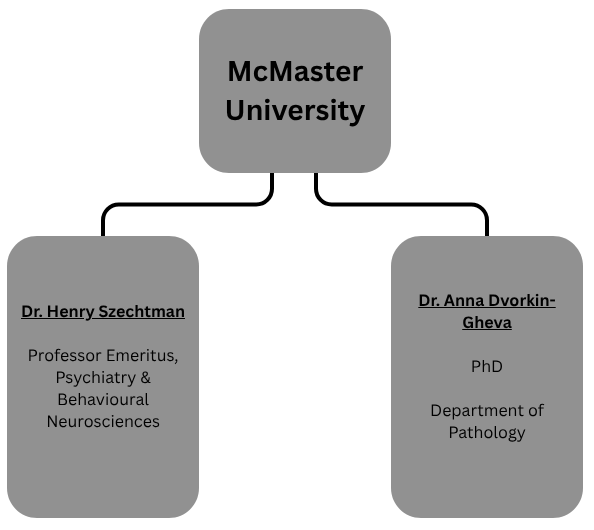
\includegraphics[width=0.5\textwidth]{2.1 Org Chart.png}
    \caption{Client Organizational Chart.}
    \label{fig:myimage}
\end{figure}

\begin{table}[H] 
    \centering
    \caption{Client and Customer Revision Dates}
    \label{tab:my_table} 

    \begin{tabular}{|l|c|} 
        \hline 
        Review Checkpoint & Date \\ 
        \hline 
        Revision 0 Design Demonstration  & Feb 2-13 2025 \\
        \hline 
        Final System Demonstration & Mar 23-29 2025 \\
        \hline 
    \end{tabular}
\end{table}
\par{Weekly meetings as well as external contact with professor will be done sporadically.}

\subsection{Customer}

\par{Since our application is intended to be \gls{open-source} and accessible to the public for free, our customers will simply be a group of end-users
of our application. Our end users will primarily involve behavioural neuroscience researchers like Dr. Henry Szechtman and Dr. Anna Dvorkin-Gheva, 
as well as graduate students and lab members, who will all benefit from the user-friendly and accessible functionality of the platform. 
Additionally we will have data scientists as customers, who will benefit from our application architecture and offered functionality for 
their purposes. Lastly, collaborating institutions and organizations from the open research community will be users of our application, 
since the application is intended to be free-use and accessible to all.\\\\}
\par{Revision Checkpoitns: See \hyperref[sec:2.1client]{2.1 Client}}


\subsection{Other Stakeholders}

\par{Other stakeholders for our project would be defined as any person or group of interest in the project outside the 
client and the customer. The first one would be our group, Gouda Engineers, as our task is to turn the project from the 
client/customer’s idea to a real product. We focus on creating documentation, building code, testing and deploying the 
software. Another stakeholder is our TA, Tiago de Moraes Machado, who is there to help our group along the way with our 
project by keeping us on track and providing feedback where it is needed. Lastly, our professor, Dr. Spencer Smith and our 
class, Capstone 4G06, would be the final stakeholders as they provide the guide and structure for building the project, 
knowledge on the topics for each step, and feedback where it is needed.}

\begin{figure}[H]
    \centering
    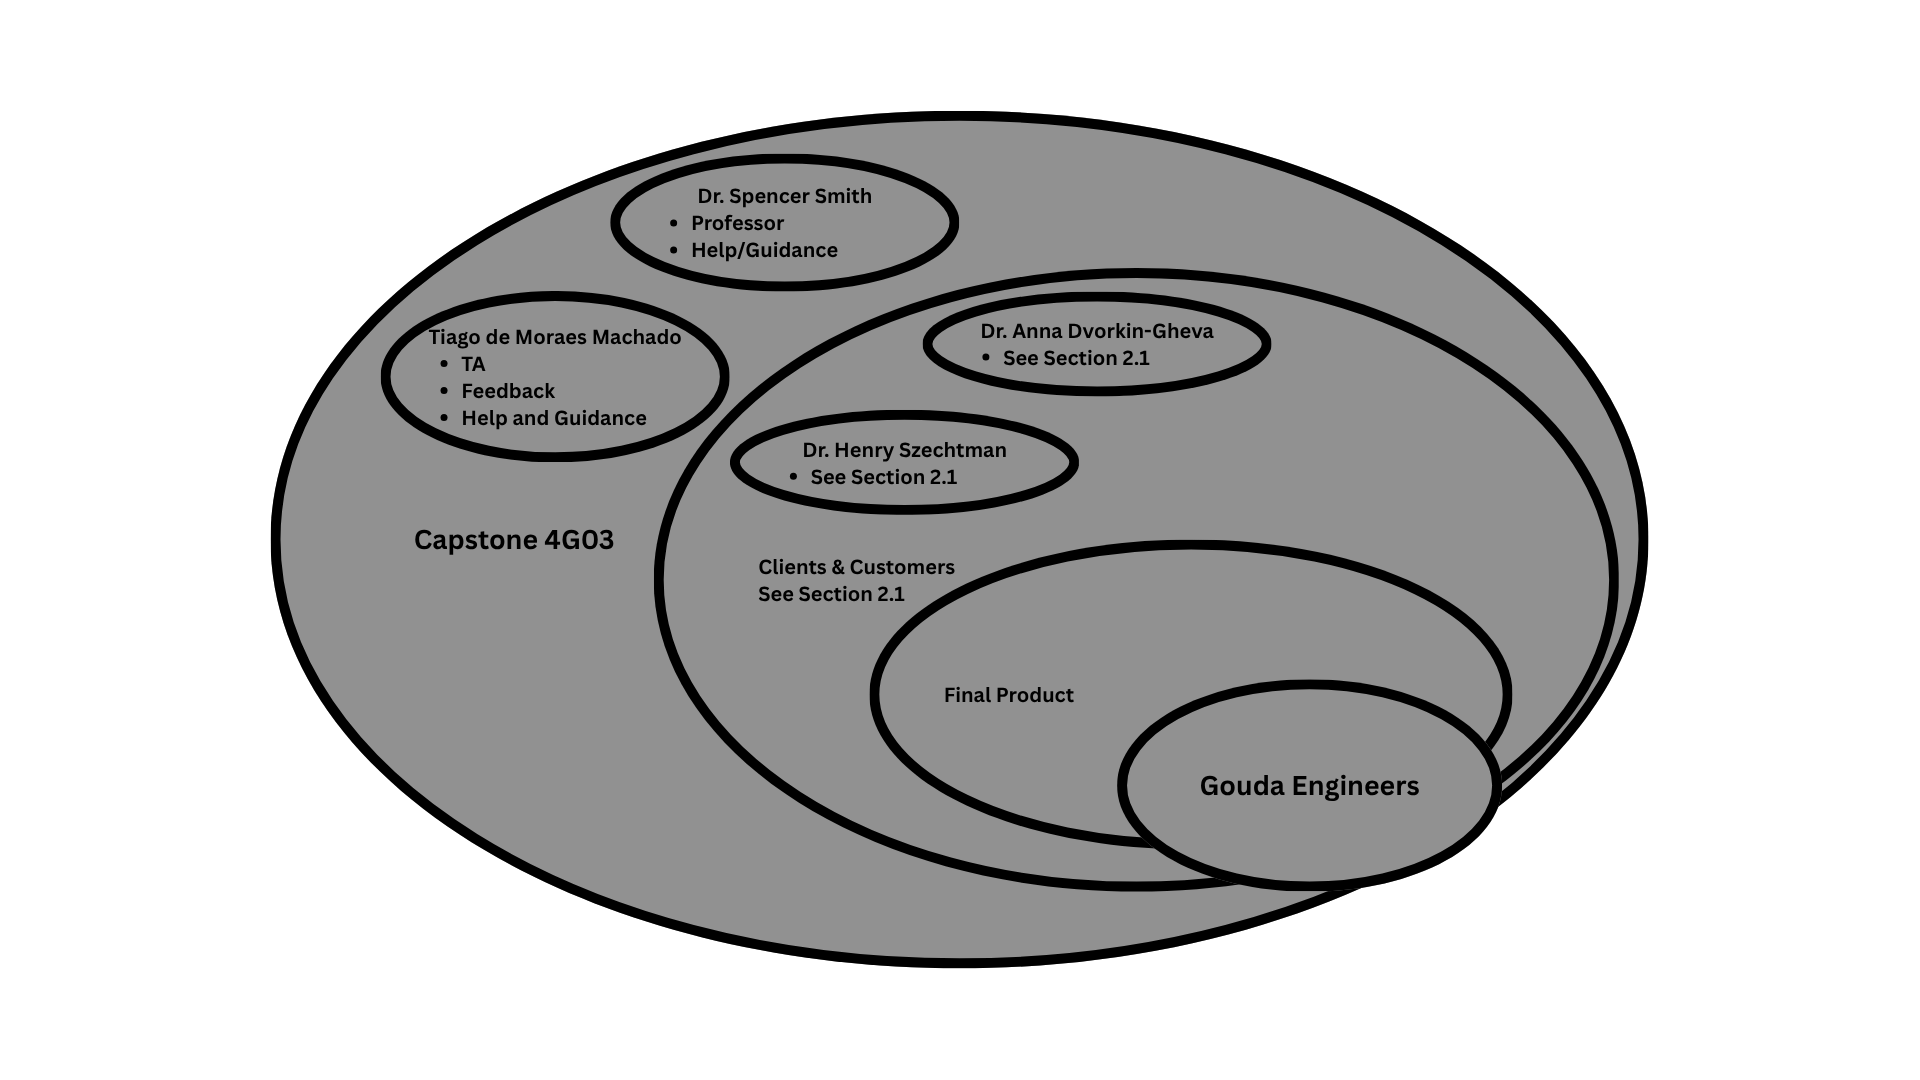
\includegraphics[width=1\textwidth]{2.3 Other Stakeholders Chart.png}
    \caption{Stakeholder Chart.}
    \label{fig:myimage}
\end{figure}

\subsection{Hands-On Users of the Project}
\label{sec:2.4handson}

The primary hands-on users of the Platform are those who will directly interact with the system for data access, analysis, and visualization. These include:

\begin{itemize}
    \item \textbf{Behavioral Neuroscientists:} Researchers who will query the dataset, visualize behavioral trajectories, and extract patterns for their studies.
    \item \textbf{Graduate and Undergraduate Students:} Students accessing subsets of the dataset for coursework, experiments, or learning purposes.
    \item \textbf{Data Scientists:} Users who programmatically analyze the data using Python or other tools, running algorithms and generating behavioral metrics.
    \item \textbf{Developers:} Individuals extending the platform or integrating it into custom workflows, running the system locally when needed.
\end{itemize}

These users will primarily interact with the system through the web interface for querying, filtering, using software tools for advanced analysis. 


\subsection{Personas}

Personas represent typical users of the system. They help in understanding user needs, goals, and interactions with the software. Each persona should include demographic information, technical expertise, motivations, and usage patterns.

\begin{itemize}
    \item \textbf{Persona Name:} Undergraduate Student
    \begin{itemize}
        \item \textbf{Role/Occupation:} Undergraduate student studying in the sciences.
        \item \textbf{Demographics:} 21 years old, undergraduate at McMaster University.
        \item \textbf{Technical Expertise:} Basic knowledge in the sciences, familiar with query interfaces, moderate computer and data analysis skills.
        \item \textbf{Goals:} Search, filter, and download records from the database for coursework or research projects.
        \item \textbf{Tasks/Responsibilities:} Navigate the website, search and filter the database, access relevant datasets.
        \item \textbf{Pain Points:} Current data is unorganized, difficult to download, and hard to query.
        \item \textbf{Usage Scenario:} Accessing the platform during a lab session to analyze data and draw conclusions.
    \end{itemize}

    \item \textbf{Persona Name:} Developer
    \begin{itemize}
        \item \textbf{Role/Occupation:} Software developer or technical enthusiast.
        \item \textbf{Demographics:} 20+ years old, undergraduate-level knowledge, comfortable with computers and software.
        \item \textbf{Technical Expertise:} High technical skill in programming, database usage, and development tools.
        \item \textbf{Goals:} Extend system features or integrate the platform into custom workflows.
        \item \textbf{Tasks/Responsibilities:} DevOps, project management, software development, testing new features.
        \item \textbf{Pain Points:} Desired features may not yet be implemented; may need to work locally to customize functionality.
        \item \textbf{Usage Scenario:} Downloading the system to run locally and develop additional features or tools.
    \end{itemize}

    \item \textbf{Persona Name:} Advisors
    \begin{itemize}
        \item \textbf{Role/Occupation:} Experienced researchers or professors overseeing the project.
        \item \textbf{Demographics:} Highly experienced in behavioral neuroscience, main stakeholders for the project.
        \item \textbf{Technical Expertise:} Advanced knowledge in the field and research methodologies.
        \item \textbf{Goals:} Ensure the system is scientifically accurate and usable for research.
        \item \textbf{Tasks/Responsibilities:} Provide guidance, make decisions on features, validate data integrity.
        \item \textbf{Pain Points:} Difficulty ensuring the data is accessible and reliable for all users.
        \item \textbf{Usage Scenario:} Reviewing the platform and verifying its usability for research purposes.
    \end{itemize}

    \item \textbf{Persona Name:} Data Scientist
    \begin{itemize}
        \item \textbf{Role/Occupation:} Researcher or analyst focused on computational analysis.
        \item \textbf{Demographics:} Graduate student or postdoctoral researcher with experience in data science.
        \item \textbf{Technical Expertise:} Proficient in Python, R, and statistical/machine learning tools.
        \item \textbf{Goals:} Analyze large-scale behavioral datasets, extract patterns, and generate insights.
        \item \textbf{Tasks/Responsibilities:} Run algorithms, process data, visualize results, integrate findings into research.
        \item \textbf{Pain Points:} Limited access to synchronized trajectory and video data; inefficient querying slows analysis.
        \item \textbf{Usage Scenario:} Programmatically accessing datasets to perform behavioral analysis and visualize results.
    \end{itemize}
\end{itemize}





\subsection{Priorities Assigned to Users}

\par{The key users for this project from the list in \hyperref[sec:2.4handson]{2.4 Hands-On Users of the Project} 
would be Behavioural Neuroscientists, Graduate and Undergraduate Students, and Developers as they are crucial 
to the long-term success of the project. The secondarcdy users would be data scientists as they will use the product 
but have little to no effect on long-term success.}

\subsection{User Participation}

\par{Estimated user participation time from \hyperref[sec:2.4handson]{2.4 Hands-On Users of the Project}:}
\begin{itemize}
    \item Behavioural Neuroscientists (1hr/week)
    \item Graduate and Undergraduate Students (1hr/week)
    \item Developers (10hr/week per developer)
\end{itemize}

\subsection{Maintenance Users and Service Technicians}

\par{Maintenance Users from \hyperref[sec:2.4handson]{2.4 Hands-On Users of the Project} :}
\begin{itemize}
    \item Developers
\end{itemize}

\par{Developers are hands-on users who must update, test, and maintain the project.}

\section{Mandated Constraints}
\subsection{Solution Constraints}
\lips
\subsection{Implementation Environment of the Current System}

\par{The OCD rat trial data set is currently hosted and accessible on the Federated Research Data Repository (FRDR), 
a Canadian national platform for research data management and sharing. The current environment has the following components:}

\begin{itemize}
    \item \textbf{User Environment}
    \begin{itemize}
        \item Users currently access datasets on FRDR through a standard web browser such as Google Chrome.
        \item No special software or hardware is needed, users can use any personal device such as their laptop or a mobile device.
    \end{itemize}
    \item \textbf{Data and Metadata Storage}
    \begin{itemize}
        \item The data set and its associated metadata are stored in FRDR's cloud-based infrastructure.
    \end{itemize}
    \item \textbf{Hosting and Maintenance}
    \begin{itemize}
        \item FRDR's cloud-based infrastructure is maintained by the Digital Research Alliance of Canada.
        \item FRDR's infrastructure incorporates redundant storage and regular data backups to ensure long-term data preservation and protection.
    \end{itemize}
    \item \textbf{Data Access and Technical Interfaces}
    \begin{itemize}
        \item Users can access and view the data set through FRDR's web portal.
        \item Data accessed through the web portal can be downloaded through links on the web page.
        \item FRDR also exposes an API specifically for data set querying and retrieval.
    \end{itemize}
\end{itemize}

\par{The following diagram is a rough outline of the form of the current system:}

\begin{figure}[H]
    \centering
    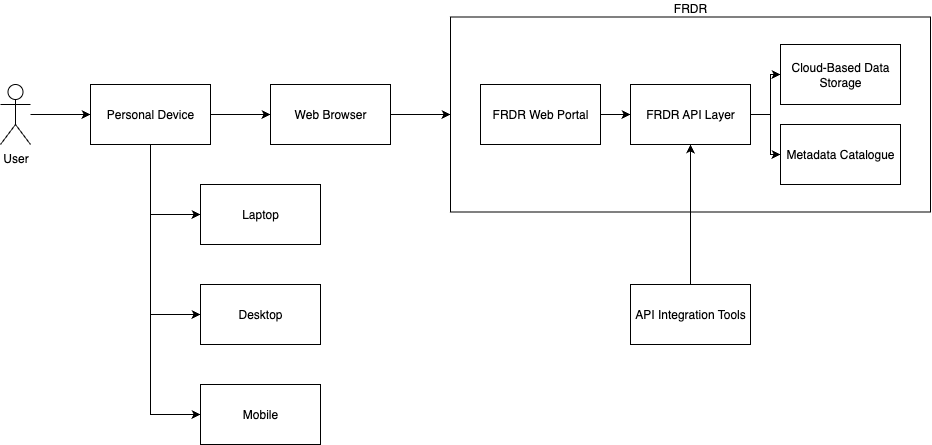
\includegraphics[width=1\textwidth]{3.2 Current System (Form) Diagram.png}
    \caption{Current System (Form) Diagram.}
    \label{fig:currentSysForm}
\end{figure}

\subsection{Partner or Collaborative Applications}
\lips

\begin{tabular}{|m{5cm}|m{10cm}|}
    \hline
    Collaborative System & System Overview \\
    \hline
    FRDR Repository & The Federated Research Data Repository is a 'bilingual bilingual publishing 
    platform for sharing and 
    preserving Canadian research data. 
    It is a curated, general-purpose repository, 
    custom built for large datasets.' This is where the data set of the rat trials is physically located
    and is dispersed across 29 independent datasets. Our system will provide a unified database schema but will
    pull data from this repository.\\
    \hline
    ratbat.mcmaster.ca & While not a directly collaborative system, this is a system made by a previous years' capstone
    team to address the same problem that our system seeks to. It will be a collaborative system in the sense that ir provides
    a reference of potential ways to approach our solution, ideas that work well and can be carried forward
    and providing visibility to shortcomings of the system will help us to avoid repeating mistakes. \\
    \hline
\end{tabular}

\subsection{Off-the-Shelf Software}

\begin{itemize}
    \item The system shall make use of the FRDR API in order to fetch the relevant data from the data set as we will not be hosting a seperate database to physically store the data for our system
    \item In the case of implementing natural language processing, an Off-the-Shelf LLM will be used to accomplish this (In other words we will not be writing our own LLM model for this purpose).
    Note that this model may need to be trained to provide results that are acceptable for our purposes.
\end{itemize}

\subsection{Anticipated Workplace Environment}

The anticipated workplace environment for the software system includes:

\begin{itemize}
    \item The workspace is defined as the computer environment where the software will operate.
    \item The system is expected to be used primarily on standard desktop or laptop computers with modern operating systems such as Windows, macOS, or Linux.
    \item Users will access the system through web browsers (e.g., Chrome, Edge, Safari) or dedicated client applications, depending on the software configuration.
    \item The system may require external software installed to run locally, such as Docker and Kubernetes.
\end{itemize}

\subsection{Schedule Constraints}

\par{Due to the nature of the capstone course, the scheduling constraints
map directly to dates in which major deliverable related to the project are due in the capstone course.
They are laid out below:}

\begin{tabular}{|m{5cm}|m{10cm}|}
    \hline
    Project Milestone & Scheduling Constraint\\
    \hline
    Software Requirements Specification & Oct 6 2025\\
    \hline
    Verification and Validation Plan & Oct 27 2025\\
    \hline
    Design Document Revision -1 & Nov 10 2025\\
    \hline
    Proof of Concept Demonstration & Nov 17-28 2025\\
    \hline
    Design Documentation Revision 0 & Jan 19 2025\\
    \hline
    Revision 0 Design Demonstration & Feb 2-13 2025\\
    \hline
    Verification and Validation Report & Mar 9 2025\\
    \hline
    Extras (Performance Report + User Manual) & Mar 9 2025\\
    \hline
    Final System Demonstration & Mar 23-29 2025\\
    \hline
    Final Documentation & April 6 2025\\
    \hline
\end{tabular}




\subsection{Budget Constraints}

\par{There is very limited budget available for this project. The department of Computing and Software at McMaster University 
will provide \$125 CAD for approved expenses. Outside of that funding, we are asked not to exceed spending of \$500 CAD
culmulatively as a team. Thus, the total budget constraints for this project are \$500 CAD in total and \$375 of our team's personal funding.}

\subsection{Enterprise Constraints}
\lips

\section{Naming Conventions and Terminology}
\subsection{Glossary of All Terms, Including Acronyms, Used by Stakeholders
involved in the Project}

\printnoidxglossary[type=SWE, title={Software Engineering Terms}]
\printnoidxglossary[type=domain, title={Domain-Specific Research Terms}]
\printnoidxglossary[type=general, title={General Terms}]



\section{Relevant Facts And Assumptions}
\subsection{Relevant Facts}

\begin{itemize}
    \item The entirety of the data set that is being worked with is available in the FRDR repository
    but is fragmented into 29 independent dats sets. 29 being the number of studies written that required relevant
    rat trials to be performed.
    \item The culmination of all the relevant data for this project is 11 terabytes and contains nearly 60,000 data objects with
    20,000 hours of video files alone.
    \item Every data object has many metadata annotations (or attributes) associated within them. In the current data hosting
    implementation on the FRDR, these are all contained in a README file that is stored in the root directory of each dataset.
    This README file has a row for each data object in the dataset and columns for each attribute.
\end{itemize}

\subsection{Business Rules}

    \par{This system does not exist within a traditional business environment and is
    rather in the realm of academia. As a result, there are no specific business rules that shape
    the requirements, the system acts as a tool in academic pursuits. Additionally, any business rules
    related to protection of information do not apply as all data being used is publicly available to
    the general public already. }

\subsection{Assumptions}

\begin{itemize}
    \item The availability and accessibility of the data in the FRDR will be upheld in definitely or at least for the lifecycle of this project.
    \item The system will not at any point, need to physically store any of the relevant data and can use the FRDR as a datastore.
    \item The API provided by the FRDR repository will be made available for our use.
    \item The query performance of the FRDR API will be reasonably efficient for our purposes.
    \item An out of the box machine learning model(s) will be available and capable of being trained in a way that it can
    perform natural language queries and categorization of rat behaviours. 
    \item API requests to the repository are independent of the user's operating system and device state. i.e. Users
    will not require any setup on their local machine to use the system.

\end{itemize}


\section{The Scope of the Work}
\subsection{The Current Situation}

\par{ The current situation currently revolves the \gls{frdr} as a means
of depositing and extracting data. Dr. Henry Szechtman and Dr. Anna Dvorkin-Gheva have
deposited the relevant data related to their work into this repository. The repository
has this data seperated into 29 distinct datasets, based on the specific study the data relates to.
Additionally, there is a large amount of metadata that is not well related to the data objects it describes
(it is stored in a readme file in each dataset which is seperate from the actual data objects). As a result, while
users are able to access all of the available data, it is very fragmented, nearly impossible to filter and search
effectively and hard to leverage for any specific research purposes. \newline\newline

Additionally, the project from last year, \href{https://ratbat.mcmaster.ca}{RatBat}, is also pulling from the \gls{frdr}
dataset using its provided API. Please see below of a graphical layout of the current situation.}

\begin{figure}[H]
    \centering
    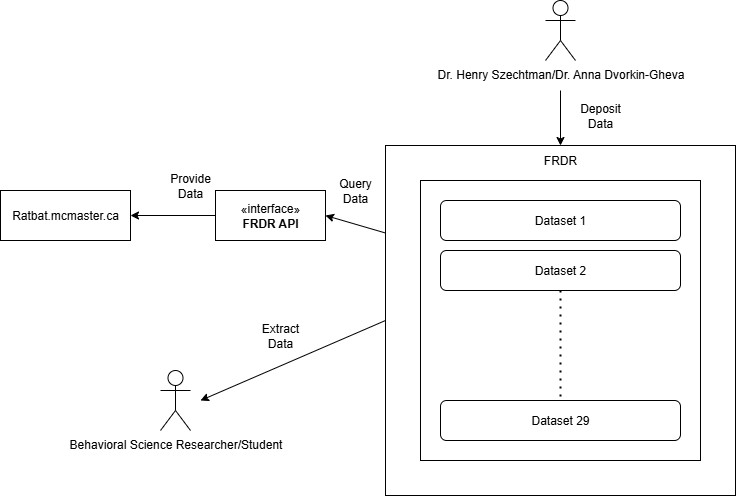
\includegraphics[width=0.8\textwidth]{6.1 Current Situation.png}
    \caption{The Current Situation}
    \label{fig:myimage}
\end{figure}


\subsection{The Context of the Work}

\begin{figure}[H]
    \centering
    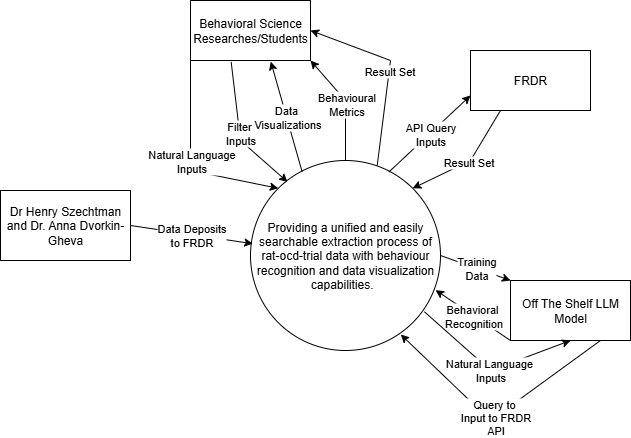
\includegraphics[width=0.8\textwidth]{6.2 Context of the Work.png}
    \caption{The Current Situation}
    \label{fig:myimage}
\end{figure}

\subsection{Work Partitioning}

The work is divided into the following components to ensure clarity, manageability, and efficient development:

\begin{itemize}
    \item \textbf{Database Design and Backend Development:} 
        \begin{itemize}
            \item Design a robust PostgreSQL database schema for behavioral data, metadata, video files, and research files.
            \item Implement REST API endpoints for data querying, filtering, and downloading.
            \item Create efficient indexing and file management systems for large-scale spatial-temporal data and video content.
        \end{itemize}
        
    \item \textbf{Interactive Web Interface:} 
        \begin{itemize}
            \item Build a React-based frontend with search and filtering capabilities.
            \item Implement natural language querying for intuitive exploration of behavioral datasets.
            \item Develop data visualization tools for plotting trajectories and behavioral metrics.
            \item Integrate synchronized video playback with trajectory data.
            \item Design user-friendly interfaces accessible to researchers without programming experience.
        \end{itemize}
        
    \item \textbf{Data Processing Pipeline:} 
        \begin{itemize}
            \item Develop Python tools to process spatial-temporal coordinate data into meaningful behavioral measures.
            \item Implement algorithms to detect key behavioral patterns (e.g., home-base behavior, checking routes, exploration metrics).
            \item Create automated analysis workflows for common research tasks.
            \item Ensure the architecture is extensible for future video analysis capabilities.
        \end{itemize}
        
    \item \textbf{NLP Integration:} 
        \begin{itemize}
            \item Integrate language model APIs to support natural language queries.
        \end{itemize}
        
    \item \textbf{Deployment and DevOps:} 
        \begin{itemize}
            \item Deploy the platform for online access with reliability and scalability.
            \item Implement caching, backup, and security measures.
        \end{itemize}
        
    \item \textbf{Documentation and Tutorials:} 
        \begin{itemize}
            \item Prepare user manuals, tutorials, and technical documentation for researchers.
            \item Provide guidelines for extending and maintaining the platform.
        \end{itemize}
\end{itemize}



\subsection{Specifying a Business Use Case (BUC)}
\lips

\section{Business Data Model and Data Dictionary}
\subsection{Business Data Model}

\begin{figure}[H]
\begin{center}
\begin{tikzpicture}[
    auto,
    umlclass/.style={
        rectangle,
        draw,
        fill=orange!10,
        text width=3.5cm,
        minimum height=1cm,
        align=left,
        font=\bfseries,
        outer sep=2pt,
        node distance=4cm
    },
    umlrelationship/.style={
        -,-,
        line width=0.8pt,
        draw=blue!70!black,
        shorten >=1pt, shorten <=1pt
    },
    multiplicity/.style={
        font=\sffamily\small,
        fill=white,
        inner sep=1pt
    },
    every node/.style={font=\sffamily\small}
]

% Classes with more attributes separated by line
\node[umlclass] (Researcher) at (0,12) {Researcher\\ \rule{\linewidth}{0.4pt}\\ + name\\ + email\\ + affiliation\\ + role};
\node[umlclass] (Supervisor) at (0,6) {Project Supervisor\\ \rule{\linewidth}{0.4pt}\\ + name\\ + department\\ + expertise\\ + contact};
\node[umlclass] (Developer) at (0,0) {Developer\\ \rule{\linewidth}{0.4pt}\\ + name\\ + skills\\ + githubID\\ + assignedTasks};

\node[umlclass] (FRDR) at (6,0) {FRDR Repository\\ \rule{\linewidth}{0.4pt}\\ + repoID\\ + description\\ + numTrials\\ + dataTypes};
\node[umlclass] (Trial) at (6,6) {Trial\\ \rule{\linewidth}{0.4pt}\\ + trialID\\ + startDate\\ + endDate\\ + injectionType\\ + notes};
\node[umlclass] (Rat) at (6,12) {Rat\\ \rule{\linewidth}{0.4pt}\\ + ratID\\ + age\\ + sex\\ + weight\\ + strain};

\node[umlclass] (Condition) at (12,12) {Condition\\ \rule{\linewidth}{0.4pt}\\ + name\\ + severity\\ + duration\\ + notes};
\node[umlclass] (Behavior) at (12,6) {Behavior\\ \rule{\linewidth}{0.4pt}\\ + behaviorID\\ + description\\ + timestamp\\ + intensity};
\node[umlclass] (Metadata) at (12,0) {Metadata\\ \rule{\linewidth}{0.4pt}\\ + key\\ + value\\ + fileType\\ + fileSize};

% Relationships
\draw[umlrelationship] (Researcher) -- (Supervisor) node[multiplicity, pos=0.1, left] {1} node[multiplicity, pos=0.9, left] {*};
\draw[umlrelationship] (Supervisor) -- (Developer) node[multiplicity, pos=0.1, left] {*} node[multiplicity, pos=0.9, left] {1};

\draw[umlrelationship] (Researcher) -- (Trial) node[multiplicity, pos=0.1, left] {*} node[multiplicity, pos=0.9, left] {*};
\draw[umlrelationship] (Researcher) -- (FRDR) node[multiplicity, pos=0.1, below left] {*} node[multiplicity, pos=0.9, above left] {*};

\draw[umlrelationship] (FRDR) -- (Trial) node[multiplicity, pos=0.1, left] {*} node[multiplicity, pos=0.9, left] {*};
\draw[umlrelationship] (Trial.east) -- (Condition.west) node[multiplicity, pos=0.1, above] {1} node[multiplicity, pos=0.9, above] {*};
\draw[umlrelationship] (Trial.north) -- (Rat.south) node[multiplicity, pos=0.1, left] {*} node[multiplicity, pos=0.9, left] {1};
\draw[umlrelationship] (Trial.east) -- (Behavior.west) node[multiplicity, pos=0.1, above] {*} node[multiplicity, pos=0.9, above] {*};
\draw[umlrelationship] (Trial.south east) -- (Metadata.north west) node[multiplicity, pos=0.1, above] {*} node[multiplicity, pos=0.9, below] {*};

\end{tikzpicture}
\end{center}
\caption{Business Data Model with Detailed Attributes}
\label{fig:myimage}
\end{figure}



\subsection{Data Dictionary}



\begin{longtblr}[
  caption = {Data Dictionary},
  label = {tab:datadictionary},
]{
  colspec = {l X l},  
  rowhead = 1,          
  hlines,               
}
\textbf{Name} & \textbf{Content/Description} & \textbf{Type} \\

% Classes
Researcher & name + email + affiliation + role & Class \\
Supervisor & name + department + expertise + contact & Class \\
Developer & name + skills + GitHub ID + assigned tasks & Class \\
FRDR Repository & repoID + description + numTrials + dataTypes & Class \\
Trial & trialID + startDate + endDate + injectionType + notes & Class \\
Rat & ratID + age + sex + weight + strain & Class \\
Condition & name + severity + duration + notes & Class \\
Behavior & behaviorID + description + timestamp + intensity & Class \\
Metadata & key + value + fileType + fileSize & Class \\

% Attributes
Trial Start Date & Start date of trial & Attribute/Element \\
Trial End Date & End date of trial & Attribute/Element \\
Injection Type & Type of drug injected & Attribute/Element \\
Rat Weight & Body weight of rat & Attribute/Element \\
Behavior Timestamp & Time of observed behavior & Attribute/Element \\
Behavior Intensity & Measure of behavior strength & Attribute/Element \\
Metadata FileType & Type of file (video, CSV, etc.) & Attribute/Element \\
Metadata FileSize & Size of file & Attribute/Element \\

\end{longtblr}

\section{The Scope of the Product}

\subsection{Product Boundary}
The product is a web-based data analysis platform designed specifically for the Dr. Szechtman Lab’s OCD behavioral neuroscience dataset. Its scope includes database design, backend services, frontend user interfaces, and data analysis pipelines to enable global researchers to access, search, analyze, and visualize rat behavioral data.

\textbf{In-Scope Features}:
\begin{itemize}
    \item \textbf{Database and Backend}: PostgreSQL schema, FastAPI endpoints, metadata management, video file management.
    \item \textbf{Frontend}: Up to date interface with advanced search/filtering, trajectory visualization, and intuitive design for non-technical researchers.
    \item \textbf{Data Processing}: Python based analysis tools for behavioral metrics, pattern detection algorithms, automated workflows, and an extensible architecture for future video-based analysis.
    \item \textbf{Deployment and Accessibility}: A fully deployed platform accessible to international researchers, with documentation, tutorials, and open-source analysis tools.
\end{itemize}

\textbf{Out-of-Scope Features}:
\begin{itemize}
    \item Direct integration with external datasets outside the OCD rat data repository.
    \item Real-time data collection from new experiments (focus is on analysis of existing dataset).
    \item Advanced machine learning video recognition (future extensibility only, not initial deliverable).
\end{itemize}

This boundary ensures the platform delivers a usable, scalable, and research-ready tool while avoiding scope creep into areas requiring separate infrastructure or regulatory compliance.

\subsection{Product Use Case Table}

\begin{table}[h!]
\centering
\begin{tabular}{|p{2.5cm}|p{2cm}|p{3.0cm}|p{3.0cm}|p{2.5cm}|}
\hline
\textbf{Use Case} & \textbf{Actors} & \textbf{Description} & \textbf{Preconditions} & \textbf{Outcome} \\
\hline
UC1: Search \& Filter Data & Researcher & Query dataset & User logged in; dataset available & Filtered dataset returned \\
\hline
UC2: Download Data & Researcher & Download trials & Dataset query completed & Files downloaded \\
\hline
UC4: Deployment \& Access & DevOps Engineer & Deploy platform online or locally & Backend/frontend configured & Platform accessible \\
\hline
\end{tabular}
\caption{Product Use Case Table}
\end{table}

\subsection{Individual Product Use Cases (PUC’s)}

\begin{description}
\item[PUC1: Search and Filter Data] The researcher searches the dataset using filters such as trial number, injection count, or behavioral pattern. The system returns relevant subsets of data.
\item[PUC2: Download Data] The researcher downloads selected subsets of trials, metadata, or video files for offline analysis.
\item[PUC3: System Deployment and Access] The DevOps engineer deploys the platform to ensure that researchers can access it globally, with necessary backend and frontend services running reliably.
\end{description}

\section{Functional Requirements}
\subsection{Functional Requirements}
\lips

\section{Look and Feel Requirements}



\subsection{Appearance Requirements}

\begin{itemize}
    \item The system shall resemble a webstore or online boutique in which possibly useful queries are packaged and presented for selection to guide 
    a non-technical user audience.
    \item The system shall not overwhelm the user with too many or overly complex visible features as to not intimidate a non-technical user audience.
    \item The system shall present the filtering and searching capabilities of the system in a way that is familiar and intuitive, such as the 
    filtering provided in an online shopping storefront.
\end{itemize}

\subsection{Style Requirements}

\par{There are no explicit style requirements for this system.}

\section{Usability and Humanity Requirements}



\subsection{Ease of Use Requirements}

\begin{itemize}
    \item The system shall have a very low ease of use floor. This floor being scrolling through
    pre-packaged query options and clicking on the one most relevant to their needs.
    \item The system shall have a reasonably low ease of use ceiling with intuitive an intuitive filtering interface
    as well as a simple natural language search interface and provided options for generating metrics and visualizations.
\end{itemize}

\subsection{Personalization and Internationalization Requirements}

\par{There are no personalization and internationalization requirements for this system.}



\subsection{Learning Requirements}

\begin{itemize}
    \item Assuming that the user is familiar with nature of the data itself, the system should
    have a learning curve of less than 30 minutes. Users shall easily be able to find and use searching
    mechanisms and querying pre-packaged and custom searches shall be very intuitive.
    \item The system shall provide options to generate available metrics or visualizations based on the queried
    data so the user does not need to learn to create their own.
\end{itemize}

\subsection{Understandability and Politeness Requirements}

\begin{itemize}
    \item The system shall hide the technical details of its queries from the users and only present naturally understandable information
    about the result set (i.e. show applied filters, natural language summary of the results).
    \item The general interface of the system should only include words that are naturally understandable to a non-technical audience (i.e. Add filters vs.
    refine query or get data vs. send database request) with the exception of technical terms in the behavioural science domain
    that are inherent to the dataset.
\end{itemize}

\subsection{Accessibility Requirements}

\par{
   The system must comply with basic web accessibility standards to ensure usability for a diverse set of researchers. All page elements must be complete with proper labelling to meet ARIA standards and ensure compatibility with assistive technology. Media including images, videos, and diagrams must offer proper alt-text and captions wherever possible. Furthermore, the system must use sufficient color contrast to support users with color blindness, and support text scaling to ensure legibility at larger font sizes.   
}

\section{Performance Requirements}

\subsection{Speed and Latency Requirements}
\begin{itemize}
    \item The system shall return all query results within 2 seconds for result sets of up to 5,000 records.
    \item All network requests shall have latency below 100 ms under normal operating conditions.
\end{itemize}

\subsection{Safety-Critical Requirements}
\begin{itemize}
    \item There are no safety-critical operations for this system, as it handles only user interface and data processing with no direct impact on human safety.
\end{itemize}

\subsection{Precision or Accuracy Requirements}
\begin{itemize}
    \item All query results shall be accurate and filtered according to user specifications.
    \item There shall be no inconsistencies between the source database and query results.
\end{itemize}

\subsection{Robustness or Fault-Tolerance Requirements}
\begin{itemize}
    \item The system shall log and report all input errors without crashing.
    \item The backend shall handle errors gracefully, storing detailed logs for debugging and monitoring purposes.
\end{itemize}

\subsection{Capacity Requirements}
\begin{itemize}
    \item The system shall support up to 250 concurrent users and handle 5,000 transactions per hour.
    \item The database and associated controllers shall be able to manage up to 11 TB of data.
\end{itemize}

\subsection{Scalability or Extensibility Requirements}
\begin{itemize}
    \item The system shall allow additional modules to be integrated without requiring major changes to existing features.
    \item Under heavy user loads, the system shall maintain at least 80\% of its performance efficiency.
\end{itemize}

\subsection{Longevity Requirements}
\begin{itemize}
    \item The system shall be designed to operate reliably for at least 5 years, with multiple teams and developers able to maintain and extend it.
    \item The system shall be compatible with any operating system when running offline.
\end{itemize}


\section{Operational and Environmental Requirements}
\subsection{Expected Physical Environment}
\begin{itemize}
    \item The system shall be able to run on a standard desktop with atleast 12 GB RAM and average processor.
    \item The software shall function correctly on Windows, macOS, and Linux operating systems.
    \item The software should be able to run in normal office environment conditions which includes temperatures between 15°C and 30°C. 
\end{itemize}

\subsection{Wider Environment Requirements}

\begin{itemize}
    \item The system shall be able to run the top three popular browers.
\end{itemize}


\subsection{Requirements for Interfacing with Adjacent Systems}

\begin{itemize}
    \item Data exchanged with adjacent systems shall use JSON format and be transmitted over HTTPS.
\end{itemize}

\subsection{Productization Requirements}
\begin{itemize}
    \item The system will use Docker and Kubernetes as it's envoirment for assebility to run on all systems.
    \item The system will provide all code changes and software updates on the GitHub Repository. 
\end{itemize}

\subsection{Release Requirements}
\begin{itemize}
    \item The system releases shall follow the versioning defined by MAJOR\#.MINOR\#.PATCH\#.
    \item The system will provide all code changes and software updates on the GitHub Repository. Code then can be pulled and tagged from the appraite GitHub release.
\end{itemize}


\section{Maintainability and Support Requirements}
\subsection{Maintenance Requirements}

\begin{itemize}
    \item Due to the open source nature of this system, maintenance shall be possible for those who are not the original developers.
    The future design documentation shall provide the necessary information to accomplish this
    \item The system shall be able to immediately accomodate the addition of new datasets into the \gls{frdr}
    assuming the contain relevant data and reflect the same structure and template as the existing datasets.
\end{itemize}

\subsection{Supportability Requirements}

\begin{itemize}
    \item The system shall be released alongside a user manual to support users in helping them understand
    the capabilities of the system and the methods for producing useful requests to the system.
    \item The system shall be self-supporting outside of the user manual as the developers will not be able
    to provide support after the project concludes and the developers graduate.
\end{itemize}

\subsection{Adaptability Requirements}

\begin{itemize}
    \item The system is expected to run on Windows 10 and later, Linux and MacOS.
    \item The system is expected to run on the top three most popular web browsers.
    \item The system is expected to maintain reasonable performance for users using devices
    with poor processing power. 

\end{itemize}

\section{Security Requirements}
\subsection{Access Requirements}

\par{There are no access requirements for our system, since it will be publicly accessible.}

\subsection{Integrity Requirements}

\par{The product shall prevent itself, the databases, and other files within it from intentional abuse.}

\subsection{Privacy Requirements}

\par{The system does not collect or use any user-related data that could be considered private and/or confidential. \newline \indent
The system does not store any personal or sensitive personal data, it only stores and presents the data which is already 
publicly available through FRDR. \newline \indent There are no privacy requirements for the system.}

\subsection{Audit Requirements}

\par{There are no audit requirements for the system. There are no data changes or transactions involved on the user's end 
and they only view already publicly available data, therefore no auditing is required.}

\subsection{Immunity Requirements}

\par{The system shall be immune to unauthorized attemps to alter data queries, inject code or exterior data, or overwhelm 
the system with an excessive ammount of requests. All inputs must be validated with network traffic being served exclusively over HTTPS, 
and users must be rate-limited to a maximum of 100 query requests per minute.}

\section{Cultural Requirements}
\subsection{Cultural Requirements}
\par{There are no cultural requirements for the system.}

\section{Compliance Requirements}
\subsection{Legal Requirements}

\par{The system must uphold all software licenses of third-party and integrated systems, as well as adhere to the MIT license defined in the project repository. \newline \indent We have consent from our 
supervisors, Dr. Henry Szechtman and Dr. Anna Dvorkin-Gheva to use their data set in the development of the project. Additionally, 
we are allowed to reference the work of the capstone group, ratbat.mcmaster.ca, which they supervised during the previous year.}

\subsection{Standards Compliance Requirements}

\begin{itemize}
    \item The platform should respect the licensing and citation requirements of \gls{frdr}. 
    \item The system must uphold all guidelines pertaining to ethical use of animal research data.
\end{itemize}

\section{Open Issues}

\begin{itemize}
    \item Verification of the specific capabilities of the \gls{frdr} \gls{api} have not yet been investigated.
    \item The extraction of the metadata of each data object is not complete and the process for extracting/referencing the metadata
    into a relational database schema has not yet completed.
    \item An investigation into the ability for an Off-the-Shelf \gls{llm} model to accurately identify compulsive behavior in the
    \gls{rat-behavioral-trials} is not yet complete.
\end{itemize}

\section{Off-the-Shelf Solutions}
\subsection{Ready-Made Products}

Several open source or commercially available products provide out of the box functionality relevant to the project. These include: 

\begin{itemize}
    \item Databases 
    \item[] Products like PostgreSQL, MongoDB, and AWS RDS are database offerings that provide robust data storage and indexing capabilities. These products meet the needs for data management at scale, but may require customization to fit the project's use. 
    \item Artificial Intelligence 
    \item[] Google's Vertex AI and the OpenAI API offer a suite of products pertaining to natural language processing and image analysis. These may be effective tools for the natural language and data processing tools central to the project, but require integration with a third party API external to the system. Specialized tools like \href{https://github.com/DeepLabCut/DeepLabCut}{DeepLabCut} offer open-source tools for animal behavioral analysis. 

\end{itemize}



\subsection{Reusable Components}

Dr. Henry Szechtman and Dr. Anna Dvorkin-Gheva possess several pre-existing software modules that can be incorporated into the system with minimal modification. This suite of tools exists as a system called \href{https://github.com/brandonc-edu/RatBAT/tree/main}{RatBat}: a previous effort to implement an interactive data platform for the OCD rodent dataset. These modules include components for interfacing with the existing dataset, as well as tools for querying the dataset. The existing \href{https://doi.org/10.1093/gigascience/giac092}{database} includes an extensive set of trials, outcomes, and metadata comprising a core reusable project component.

\subsection{Products That Can Be Copied}


The client has provided several resources to serve as references for the implementation of the system. One similar interface is the \href{https://portal.gdc.cancer.gov/analysis_page?app=CohortBuilder&tab=general_diagnosis}{GDC Data Portal} which provides a querying interface that may be replicated by the system. Furthermore, the client expressed a goal of incorporating a user-friendly, e-commerce-like catalogue interface, citing retailers such as \href{https://amazon.ca}{Amazon} as a reference for user interface design. 


\section{New Problems}
\subsection{Effects on the Current Environment}

The new system will be developed from the ground up, there is no current implementation environment to affect. The only existing system that will be interacted with is the FRDR repository which provides
a stable API for accessing the relevant data sets that will be used and will thus be unaffected by any developments made.

\subsection{Effects on the Installed Systems}

\par{ The 'installed system' that concerns this project is the FRDR repository as it will be used as a part of the system to provide the required functionality. The interactions between the new system and
the FRDR repository will all be through a REST API that the FRDR provides. As a result no effects or conflicts are anticipated, although this conclusion operates under the assumption that the provided
API is sound. }


\subsection{Potential User Problems}

\par{An important note to make about the project is that it is not a mandatory replacement for the existing data set and infrastructure 
available through FRDR. Users besides the commissioners of our project, our supervisors, can simply keep using the existing system 
if that better suits their needs. \newline \indent The comissioners of our project, and external users of the project due to its public 
availability, could have a potential issue with the Natural Language Processing (NLP) used in querying raw data files. Since natural language 
will be converted to a query statement using an AI model, it cannot be guaranteed the model will be accurate 100\% of the time when 
creating these queries from natural language.}

\subsection{Limitations in the Anticipated Implementation Environment That May
Inhibit the New Product}
\lips
\subsection{Follow-Up Problems}
\lips

\section{Tasks}
\subsection{Project Planning}
\lips
\subsection{Planning of the Development Phases}
\lips

\section{Migration to the New Product}
\subsection{Requirements for Migration to the New Product}

\par{There are no requirements for migration to the new product other than that the user must familiarize themselves with the new domain and UI if they are used to using the FRDR repository.}


\subsection{Data That Has to be Modified or Translated for the New System}

\par{The new system will take the raw data directly from the FRDR repository and present it to users. There are use cases in which the data will be processed for the purposes 
     of producing metrics or visualizations which is relevant to the functional requirements rather than this section. Thus, no data needs to be modified or translated for this new system.}

\section{Costs}

\par{There are no costs associated with the development of this project.}

\section{User Documentation and Training}
\subsection{User Documentation Requirements}

\begin{itemize}
    \item The system shall be released alongside a user manual guiding users through the possible inputs they have access to, how to properly execute them as well as the corresponding outputs that will be produced as a result. The inputs that 
    will be over: querying pre-packaged result sets, generating custom filters, natural language searching, producing behaviour metrics, producing data visualizations.
\end{itemize}

\subsection{Training Requirements}

\par{ There are no explicit training requirements for this system. The interface should be sufficiently intuitive and the user manual must be interpretable by a non-technical user if they need to learn specific functions.
No explicit training will be needed }

\section{Waiting Room}
\lips

\section{Ideas for Solution}
\lips

\newpage{}
\section*{Appendix --- Reflection}

The purpose of reflection questions is to give you a chance to assess your own
learning and that of your group as a whole, and to find ways to improve in the
future. Reflection is an important part of the learning process.  Reflection is
also an essential component of a successful software development process.  

Reflections are most interesting and useful when they're honest, even if the
stories they tell are imperfect. You will be marked based on your depth of
thought and analysis, and not based on the content of the reflections
themselves. Thus, for full marks we encourage you to answer openly and honestly
and to avoid simply writing ``what you think the evaluator wants to hear.''

Please answer the following questions.  Some questions can be answered on the
team level, but where appropriate, each team member should write their own
response:


\begin{enumerate}
  \item What went well while writing this deliverable? 
  \item What pain points did you experience during this deliverable, and how did
  you resolve them?
  \item How many of your requirements were inspired by speaking to your
  client(s) or their proxies (e.g. your peers, stakeholders, potential users)?
  \item Which of the courses you have taken, or are currently taking, will help
  your team to be successful with your capstone project.
  \item What knowledge and skills will the team collectively need to acquire to
  successfully complete this capstone project?  Examples of possible knowledge
  to acquire include domain specific knowledge from the domain of your
  application, or software engineering knowledge, mechatronics knowledge or
  computer science knowledge.  Skills may be related to technology, or writing,
  or presentation, or team management, etc.  You should look to identify at
  least one item for each team member.
  \item For each of the knowledge areas and skills identified in the previous
  question, what are at least two approaches to acquiring the knowledge or
  mastering the skill?  Of the identified approaches, which will each team
  member pursue, and why did they make this choice?
\end{enumerate}


\section{Nathan Perry Reflection:}

\begin{enumerate}
  \item What went well while writing this deliverable? 

  \par{ Understanding the expectations for this deliverable went well, especially relative to the previous deliverable. In the goals and problem statement
  document, I felt that we had a general idea of what we needed to do but not a concrete guide. Using the Volere template, we were able to find very helpful
  documentation which provided an overview of specifically what was expected to be put in each section. This made writing the document feel much more structured
  and provided confidence we were on the right track, especially since the document itself gives very little to go off of aside from section titles.}

  \item What pain points did you experience during this deliverable, and how did
  you resolve them?

  \par{ Far and away the biggest and nearly only pain point for this deliverable was the delegation of work among the members. A few of us like the frontload
  the effort over the deadline window while others like to backload the effort and thus, a few members ended up starting early and needing to take on more
  than their fair share of tasks as an inevitable scramble to complete the deliverable ensued. To try to resolve this, the members who did not start earlier offered
  to take on the rest of the work, telling the others they don't need to continue to contribute. This was somewhat helpful but the deliverable needs to get done
  so everyone ended up helping to some extent anyways. In the future, we decided to resolve this by delegating tasks before work begins. For the SRS
  we used a 'take-as-you-go' approach to issues whereas from now on we will be assigning everything ahead of time. }


  \item How many of your requirements were inspired by speaking to your
  client(s) or their proxies (e.g. your peers, stakeholders, potential users)?

\par{I cannot give a concrete number of requirements that were inspired by speaking to our client but we did have a meeting with Dr. Henry Szechtman
in the week leading up to the writing of our SRS document. The biggest requirement that he directly inspired was the idea to pre-package queries
and display them like a webstore so that users who may not even know exactly what they are looking for can derive value from our system. Furthermore,
our filtering requirements were guided by a reference website created by the National Cancer Institute which
was provided by our client as a reference. \href{https://portal.gdc.cancer.gov/analysis_page?app=CohortBuilder&tab=general.}. Requirements
to make the project maintainable by people other than the original developers and to be open source was also inspired by our client meeting as Dr. Szechtman wants the
project to carry on after we graduate.
}

  \item Which of the courses you have taken, or are currently taking, will help
  your team to be successful with your capstone project.

  \par{ Our project is very multi disciplinary as it is a full stack project and thus plenty of what we learned will go into
  our development. First and foremost, our databases class will provide the knowledge needed to design a database schema as a foundation
  for our entire system. Additionally, the Human-Computer interfaces class we are currently taking will be helpful in creating a user interface
  that is approachable for a non-technical audience. Furthermore, all of the very coding heavy courses including object oriented programming, system
  design and software development will help us to implement the core business logic of the application and to connect the different components.
  Finally, I will add that the our data structures class will help us to efficiently store, package and represent the data objects being transmitted
  in our system. }
\end{enumerate}

\section{Timothy Pokanai Reflection}

\begin{enumerate}
  \item What went well while writing the deliverable?
  \par{I would say that we were able to smoothly and consistently deliver our preliminary SRS document. What I mean is as we worked throughout the deliverable 
  our individual ideas and interpretations of our project description, through the forms of requirements, were aligned and consistent. To be fair we may have had 
  a commit or two where something I wrote was modified to better suit the context of our project, but that was the only occurence in terms of peer performed changes. 
  I would attribute our team's ability to work individually with seamless integration to the fact that we all acquired a great grasp of the scope of the project and 
  the constraints associated with it early on. A lot of this can be attributed to our supervisors with their involvement and a bit from the public nature of the project.}

  \item What pain points did you experience during this deliverable, and how did
  you resolve them?
  \par{What caused some turbulence while working on this deliverable was not related to the deliverable at all, it was how we delegated work throughout our team. 
  We used a first-come-first-serve approach when it came to picking up issues related to our deliverable, which had both its pros and cons. It allowed some 
  members of our team to pick what they wanted to do earlier on and often times they would do it early. This allowed some members to complete their 
  work earlier on in the project timeline which is definitely a pro. On the flip side, members that start their work later on don't have as much flexibility in 
  their choice of work issues. This resulted in an imbalance of workload between group members where some would be left with multiple issues with more weight in 
  work when compared to previously completed issues, and at times people who did their share of work needed to complete extra for the sake of time. Our resolution plan 
  moving forward is to delegate tasks in a different manner, which will be dividing sections so everyone has equal weight in work before anyone starts working 
  on a deliverable.
  }

  \item How many of your requirements were inspired by speaking to your
  client(s) or their proxies (e.g. your peers, stakeholders, potential users)?
  \par{Its hard to keep track of how many requirements exactly were inspired by our conversations with our clients and their proxies, but I'll provide the 
  general requirement section names which were mostly or fully completely based on our discussions. Our mandated constraints were heavily based on context 
  provided to us about the current and future system implementation. The functional requirements we created were directly inspired by what features our clients wanted 
  to see us deliver with the project. The requirement sections related to the usability and user experience of the software, which were look and feel 
  and usability and humanity requirements, were inspired by our clients goals of creating easy-to-use and globally accessible software. Lastly, since our clients are 
  actively involved with the current system in place, we were able to clearly interpret their requirements in the operational and environmental domain, 
  as well as security and compliance requirements.}

  \item Which of the courses you have taken, or are currently taking, will help
  your team to be successful with your capstone project.
  \par{Some elements from the project-based courses, most notably 1P13 and 2PX3, will definitely help with the pacing and iterative nature in terms of development and 
  documentation of our project. Also from those project based courses, we can use principles we have learned about working in a group and doing presentations which will 
  be more prevalent further in the project timeline. On the topic of workflows and development cycles, I think we will need to adopt one or two development cycles like 
  Agile Methodology coupled with Test Driven Development for example. We have each had much practice with some kind of development cycle from our Software Design I and III 
  courses where we focused on building larger-scale software during a time period, and we will definitely need to apply what we have learned from those for our documentation 
  and development. Furthermore, one of our main focus points for this project is to create a user friendly and accessible interface for users of our software. We are all 
  currently in a Human Computer Interfaces class where we will need to apply what we learn about user elicitation, design, and experience. Lastly, our project will heavily rely 
  on data that will be visualized and possible pre-processed by users. This will be a perfect opportunity to apply our learnings from our Database Design course and our Concurrent 
  System Design course, both of which go hand-in-hand when designing efficient, scalable, and safe databases.}
\end{enumerate}

\section{Jeremy Orr Reflection:}

\begin{enumerate}
 \item What went well while writing this deliverable?

    \par{I think our team worked effectively to complete a large and detailed document in an organized manner. We communicated clearly and consistently throughout the process, which helped us stay aligned with our goals. Personally, I was able to complete my assigned sections early and efficiently. As a group, we also did a good job discussing challenges openly and collaborating to resolve them.}

    \par{One specific event that went particularly well was our collaborative editing session before submission. During that session, we reviewed the entire document together, finalized remaining sections, and made meaningful improvements. This not only strengthened the overall quality and consistency of the deliverable but also ensured that everyone’s contributions were well integrated. Overall, our teamwork and communication during that session demonstrated how effectively we could work together under a deadline.}

  \item What pain points did you experience during this deliverable, and how did you resolve them?

    \par{One of the main challenges we faced was dividing the work fairly among team members. Initially, we used a first-come, first-served approach, which led to an uneven distribution of tasks. Additionally, I accidentally started working on a section that a team member had already begun, which caused some inefficiency and duplicated effort.}

    \par{To resolve these issues, we discussed a more structured approach for future work, agreeing to evenly divide tasks before starting on a deliverable. For my specific issue, I committed to reviewing team assignments and communicating with teammates before beginning work on any section, ensuring that efforts are coordinated and that overlap is avoided. This experience highlighted the importance of proactive communication and clear task assignment in collaborative projects, which we will carry forward into future deliverables.}

  \item How many of your requirements were inspired by speaking to your client(s) or their proxies (e.g., your peers, stakeholders, potential users)?

    \par{The primary requirement that was influenced by discussions with our client was clarifying the specific scope and objectives of the project. We held multiple meetings with the clients, during which they shared numerous ideas for future extensions and potential features. These conversations were important to ensure that our team focused only on the deliverables required for the current project and did not extend into future scope items. Other than clarifying the project scope, there were few additional requirements that needed direct input from the client, as much of the remaining work was based on established technical objectives and user needs identified through our research.}

  \item Which of the courses you have taken, or are currently taking, will help
  your team to be successful with your capstone project.

    \par{I believe that several courses will help our team succeed in this capstone project. These include SFWRENG 2AA4: Introduction to Software Development, SFWRENG 3RA3: Software Requirements, SFWRENG 3A04: Software Testing, and the Software Architecture course. These courses have provided us with great knowledge in software development practices, requirement gathering, system design.}


\end{enumerate}

\end{document}
